\documentclass[10pt,letterpaper]{article}
% Add a bunch of useful math, font, and symbols
\usepackage{amsfonts}
\usepackage{amsmath}
\usepackage{amssymb}

% English support
\usepackage[english]{babel}

% Citation
\usepackage[superscript]{cite}

% Better enumerate and itemize
\usepackage{enumitem}

% Better control of headers and footers
\usepackage{fancyhdr}

% Floating objects like figures and tables
\usepackage{float}

% Page layout and dimensioning
\usepackage[margin=1in]{geometry}

% Basic color, graphics and text manipulation 
\usepackage{graphicx}

% Use Helvetica typeface
\usepackage[scaled]{helvet}
\renewcommand\familydefault{\sfdefault} 
\usepackage[T1]{fontenc}

% Cross-referencing hyperlinks
\usepackage{hyperref}

% Line break for long URLs
\usepackage{breakurl}

% Accept utf-8 input encoding
\usepackage[utf8]{inputenc}

% Make indexes
\usepackage{makeidx}

% Microtype (apparently makes the typographics stuff better)
\usepackage{microtype}

% [Disabled] multi-column writing
% \usepackage{multicol}

% English ordinal counting (1st, 2nd, etc.)
\usepackage{nth}

% Long table
\usepackage{longtable}

% Paragraph skip - adds extra lineskip spacing
\usepackage{parskip}
\setlength{\parskip}{0.7\baselineskip plus 2pt}

% Add ability to set space between lines
\usepackage{setspace}

% S.I. units
\usepackage{siunitx}

% Subcaptions for subfigures
\usepackage{subcaption}

% Include svg graphics
\usepackage{svg}

% Drawing graphics
\usepackage{tikz}

% Subsubsubsection
\usepackage{titlesec}
\setcounter{secnumdepth}{4}
\titleformat{\paragraph}
{\normalfont\normalsize\bfseries}{\theparagraph}{1em}{}
\titlespacing*{\paragraph}
{0pt}{3.25ex plus 1ex minus .2ex}{1.5ex plus .2ex}

% Custom titles
\usepackage{titling}

% Url
\usepackage{url}

\RequirePackage[figure,table]{totalcount}


% Custom definitions
\newcommand{\doctitle}{List of Deliverables}
\newcommand{\docsubtitle}{Computing Platform Multirotor with FPGA Hardware Acceleration Applications}

% Custom commands
\newcommand{\ts}{\textsubscript}	% Subscript command %


\renewcommand{\revisionnum}{1.1}
% Use hyphans to break up urls
\def\UrlBreaks{\do\/\do-}

% PDF and href setup
% Hyper ref
\hypersetup{
	colorlinks=true,
	citecolor=black,
	linkcolor=black,
	filecolor=black,
	urlcolor=blue,
	pdftitle={\@title},
	bookmarks=true
}
\urlstyle{same}
% Page headings
\pagestyle{fancy}
\fancyhead[L]{\MakeUppercase{CPEN/ELEC 491}}
\fancyhead[C]{\textbf{\doctitle}}
\fancyhead[R]{Mieszko Lis, PhD}
\fancyfoot{}
\fancyfoot[C]{Non-Confidential}
\fancyfoot[R]{\thepage}

% No paragraph indent
\parindent 0ex

% Meta
\author{
	Deutsch, Peter &
	\textit{me@peterdeutsch.ca}
	\\
	He, Muchen &
	\textit{m.he@alumni.ubc.ca}
	\\
	Hsueh, Arthur &
	\textit{ah11962@outlook.com}
	\\
	Wang, Meng &
	\textit{wzfftxwd@gmail.com}
	\\
	Wilson, Ardell &
	\textit{ardellw96@gmail.com}
}
\title{\doctitle}
\date{\today}
\makeatletter
\renewcommand{\maketitle}{
	\bgroup
	\setlength{\parindent}{0pt}
	\begin{flushleft}
		% Top spacing
		\vspace*{0.5in}

		% Team logo
		
\includegraphics[scale=0.4]{../assets/capstonelogo1.png}
		\vspace*{0.25in}

		% Title
		\textbf{\Huge{\@title}}\\
		\hrulefill

		% Subtitle
		\textbf{\huge{\docsubtitle}}
		
		\vspace*{0.5in}

		% Course number and team
		\textbf{\Large{CPEN/ELEC 491 Capstone Team 109}}\\
		\hspace*{0.1cm}
		\begin{tabular}[h]{|ll}
			\@author
		\end{tabular}

		\vspace*{0.25in}

		\textbf{\Large{Mieszko Lis, PhD}}\\
		\hspace*{0.1cm}
		\begin{tabular}[h]{|ll}
			Electrical and Computer Engineering, The University of British Columbia
		\end{tabular}

		\vfill
		
		% Date
		\large{Revision 1.0 -- \@date}
		\vspace*{0.5in}

		% Logo
		\hspace*{-0.3cm}
\includegraphics[scale=0.5]{../assets/ece_logo.pdf}

	\end{flushleft}
	\egroup
}
\makeatother

% Begin Document
\begin{document}
% Title Page
\begin{titlepage}
	\maketitle
\end{titlepage}


\renewcommand{\thepage}{\roman{page}}
\setcounter{page}{1}

% Revision history
\backgroundsetup{
	scale=1,
	color=black,
	opacity=0.3,
	angle=0,
	contents={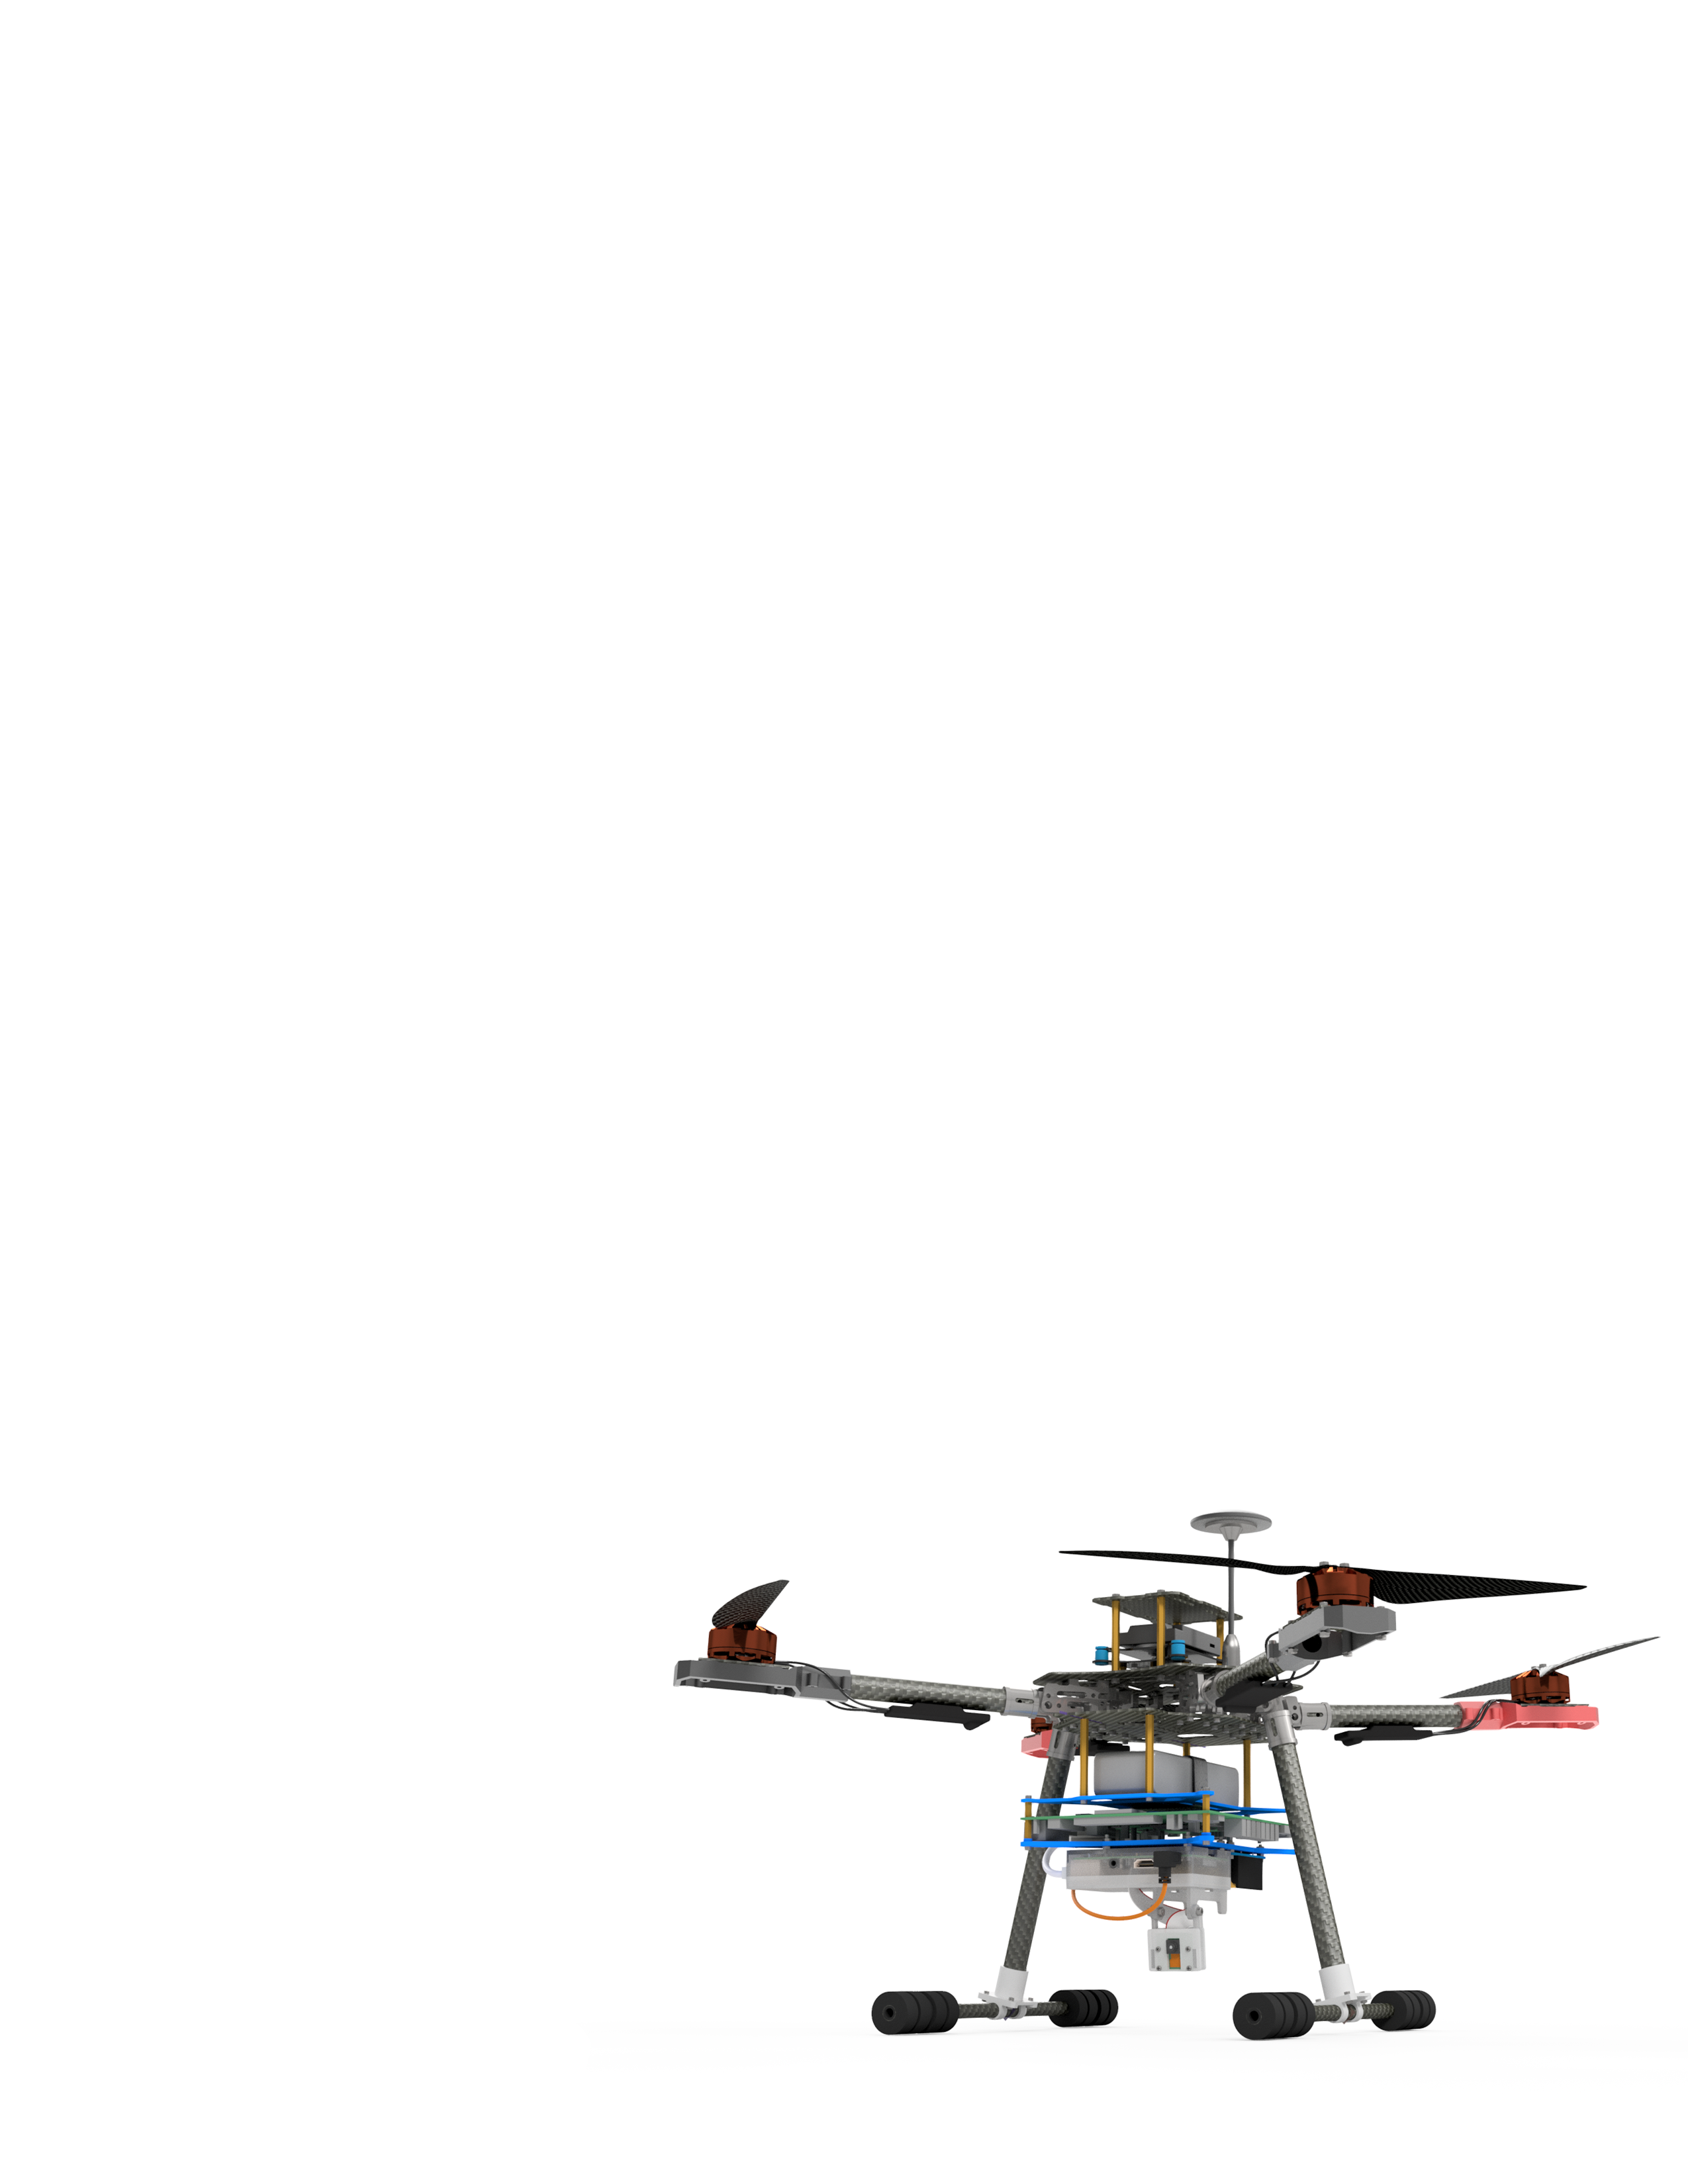
\includegraphics[height=\paperheight,width=\paperwidth]{../assets/render2bg}}
}
\BgThispage
%\thispagestyle{empty}
\section*{Revision History}
The full revision history and commited changes of the document can be found in the git repository history: \href{https://github.com/Capstone-Skynet/Capstone-Skynet.github.io}{https://github.com/Capstone-Skynet/Capstone-Skynet.github.io/commits/master}.

\begin{table}[H]
\begin{tabular}{*{4}{l}p{0.5\linewidth}}
\hline
Version \# & Initials & Release Date & Changeset & Changes Made \\ \hline

0.0 & PD & 2019-10-11 & \texttt{660e001} & Initial skeleton of the document.\\
0.1 & MH & 2019-10-11 & \texttt{6af9e8a} & Populate initial document with draft content required for Milestone I.\\
0.2 & PD & 2019-11-23 & & Initial framework for test descriptions created.\\
0.3 & MW & 2019-11-24 & & First set of tests added.\\
1.0 & PD & 2019-11-25 & & General clean-up and release for Milestone II.\\
1.1 & AH & 2020-02-09 & & Added Full System Tests \\

 & & & \\ \hline
\end{tabular}
\end{table}
\clearpage

% Table of contents
\setcounter{secnumdepth}{3}
\tableofcontents

% Roman numeral page numbers


% Terms and Abbreviations
\thispagestyle{empty}

\section*{Terms and Abbreviations}

Technical terms and abbreviations dictionary go here.

\begin{tabular}[h]{rp{0.75\linewidth}}
    \hline
    \textbf{Term} & \textbf{Definition}\\
    \hline

    ANN & Artificial Neural Network, or simply ``Neural Network'', is a data processing model modeled after neuron interactions. The process consists of forward propagation using several matrix multiplications.\cite{ann}\\
    ASIC & Application-specific Integrated Circuits.\\
    CNN & Convolutional neural network are neural networks that is especially useful for image classification.\cite{cnn} \\
    ECE & Department of Electrical and Computer Engineering at the University of British Columbia.\\
    FPGA & Field-Programmable-Gate-Arrays, ``programmable'' hardware that allows ASIC-like performance with software-like turn-around time and flexibility.\\
    GPU & Graphics Processing Unit, a discrete piece of hardware designed to accelerate graphic-intensive or other parallel computing tasks.\\
    LOS & Line-of-sight.\\
    ML & Machine learning.\\
    Multirotor & An unmanned vehicle with multiple engines. \\
    OTS & Off-the-shelf, or commercially available/purchasable \\
    PID / PID Controller & Proportion-Integral-Derivative controllers is the most common control algorithm for precise and accurate movement, as well as to compensate external forces.\cite{pid}\\
    RNN & Recurrent neural networks are neural networks where the output depends on previous computations, essentially consists of memory.\cite{rnn}\\
    RX & Receiver.\\
    TC & Transport Canada.\\
    TX & Transmitter.\\
    YOLO & You-Only-Look-Once is a fast ML algorithm that detect objects but is unlike CNN nor RNN.\cite{yolo}\cite{yolo-2}\\
     & \\

    \hline

\end{tabular}


% List of figures and tables
\iftotalfigures
\addcontentsline{toc}{section}{\listfigurename}
\listoffigures
\fi
\iftotaltables
\addcontentsline{toc}{section}{\listtablename}
\listoftables
\fi

\newpage

% Set page and section counter
\renewcommand{\thepage}{\arabic{page}}
\setcounter{page}{1}
% TODO: fill out all the sections
% if the sections gets too long, move them to a separte .tex document
\section{About This Document}
This document outlines the full list of deliverables presented to the client at the end of the project.

\section{List of Deliverables}
\subsection{Hardware Artifacts}
\subsubsection{Computing Platform Artifacts}
\begin{itemize}
\item 1 -- Raspberry Pi 4
\item 1 -- Micro-SD Card (for Raspberry Pi)
\item 1 -- Raspberry Pi Camera Module (5 MP)
\item 1 -- USB-C to Mains Adapter
\item 1 -- Ethernet Cord (10 ft)
\item 1 -- Zedboard
\item 1 -- SD Card (for Zedboard)
\item 1 -- 12V Barrel Plug to Mains Adapter
\item 2 -- Micro-USB to USB-A Cable
\end{itemize}

\subsubsection{Multirotor Artifacts}

\subsection[Document Artifacts]{Document Artifacts\footnote{All referenced documents can be found at \url{https://github.com/Capstone-Skynet/Capstone-Skynet.github.io}}}

\begin{itemize}

\item Requirements Specification
\item Design Specification
\item Validation Specification and Results
\item Operations, Maintenance, and Upgrades Specifications
\item List of Deliverables
\end{itemize}

\subsection{Other Artifacts}
\begin{itemize}
\item Demonstrative Video
\item Oral Presentation
\item Project Repositories
\begin{itemize}
\item Documents and Meeting Notes Repository ({\url{https://github.com/Capstone-Skynet/Capstone-Skynet.github.io}})
\item Source Code Repository ({\url{https://github.com/Capstone-Skynet/Integration}})
\end{itemize}
\end{itemize}

% Appendix (uncomment to enable appendix)
% \clearpage
% \appendix
% \section{Appendix name}\label{appendix:sample-appendix}
% Content here

\end{document}